% !TEX root = knottedMain.tex
\documentclass[varwidth=\maxdimen]{standalone}

\usepackage{mathtools,amssymb,mathrsfs,dutchcal,upgreek,faktor,accents,etoolbox,multicol}
\usepackage[dvipsnames]{xcolor}
\definecolor{mygreen}{RGB}{	8,156,79 }
\usepackage{tikz,tikz-cd}
\usetikzlibrary{patterns,knots,arrows.meta,decorations.markings}
\tikzset{>={Straight Barb[scale=0.85]}}
\tikzcdset{
  cells={font=\everymath\expandafter{\the\everymath\displaystyle}},
  arrow style=tikz,
  diagrams={>={Straight Barb[scale=0.85]}},
  every label/.append style = {font = \small}
}



\begin{document}

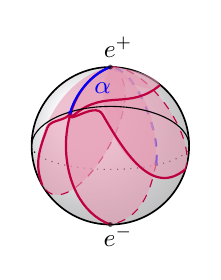
\begin{tikzpicture}[fill opacity=0.6]
    \begin{scope}
        \clip (3.95,-1.35) rectangle (6.05,1.5);
        \foreach \y in {5}{
        \shade[ball color=blue!3!white,opacity=0.4] (\y,0) circle (1cm);
        \draw[dotted] (\y-1,0) arc (180:360:1cm and 0.3cm);
        \draw[semithick] (\y,0) circle (1cm);
        }
        \draw[opacity=1,blue,dashed,thick]
            (5.58,-.22)
            to[out=80,in=-5,distance=0.35cm]
            (5,1);
        \fill[blue]
            (5.58,-.23) circle (0.8pt);
            
            % \fill[purple!40] 
            %     (4.03,0.21) to[in=-175,out=65,distance=0.45cm](5,1) to[out=-40,in=-110,distance=0.57cm] (4.03,0.21);
            \fill[purple!40]
                (4.135,-0.5) to[in=-170,out=110,distance=0.6cm]
                (5,1) to[out=-25,in=-60,distance=0.7cm] (4.135,-0.5);
\draw[purple,dashed]
    (5,1) to[out=-25,in=-60,distance=0.7cm] (4.135,-0.5);
            \fill[purple!40]
                (5,-1) to[in=-160,out=160,distance=0.8cm]
                (5,1) to[out=-20,in=10,distance=0.8cm] (5,-1);
\draw[purple,dashed]
    (5.58,-.22) to[out=-100,in=10,distance=0.38cm] (5,-1); 
                % \fill[purple!40]
                %     (5.52,-0.85) to[in=-130,out=180,distance=0.75cm]  
                %     (5,1) to[out=-15,in=35,distance=0.8cm] (5.52,-0.85);
                \fill[purple!40]
                     (5.95,-0.3) to[in=-120,out=-140,distance=0.7cm] 
                     (5,1) to[out=5,in=70,distance=0.45cm] (5.95,-0.3);
 \draw[purple,dashed]
    (5,1) to[out=5,in=70,distance=0.45cm] (5.95,-0.3);                
                % \fill[purple!40] 
                %     (5.95,0.3) to[in=-100,out=-150,distance=0.4cm] 
                %     (5,1) to[out=0,in=100,distance=0.25cm] (5.95,0.3);
                \fill[purple!40] 
                    (5,1) to[out=-50,in=-140,distance=0.2cm] 
                    (5.63,0.77) to[in=0,out=110,distance=0.15cm] (5,1);

        \draw[purple,thick] 
            (5,1) to[out=-160,in=160,distance=0.8cm] (5,-1);
        \draw[purple,thick] 
            (4.49,0.42) to[out=-110,in=70,distance=0.12cm] 
            (4.2,0.23) to[out=-110,in=110,distance=0.3cm]
            (4.135,-0.5);
        % \draw[purple,thick] 
        %     (4.5,0.4) to[out=-100,in=180,distance=0.5cm] (5.52,-0.85);
        \draw[purple,thick] 
            (4.49,0.42) to[out=-110,in=120,distance=0.2cm]
            (4.9,0.4) to[out=-60,in=-140,distance=0.55cm] (5.95,-0.3);
        % \draw[purple,thick] 
        %     (4.5,0.42) to[out=-80,in=-150,distance=0.4cm] (5.95,0.3);
        \draw[purple,thick] 
            (4.49,0.42) to[out=-110,in=-140,distance=0.05cm] 
            (4.55,0.4) to[out=40,in=-140,distance=0.5cm] 
            (5.63,0.77);


        \draw (4,0) arc (180:0:1cm and 0.5cm);


        \draw[opacity=1,blue,thick]
            (5,1) to[out=-160,in=75,distance=0.25cm]
            (4.49,0.42)
            (4.9,0.73) node{\small$\alpha$} ;
        \fill[blue]
            (4.49,0.42) circle (0.8pt);

        \fill 
            (5,-1) circle (0.9pt)
            (5,1) circle (0.9pt);

        \draw[opacity=1]
            (5.1,-1.15) node{\small$e^-$}
            (5.1,1.25) node{\small$e^+$};
    \end{scope}
\end{tikzpicture}~\qquad
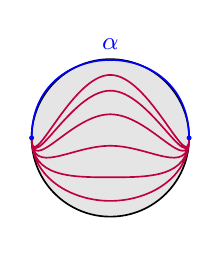
\begin{tikzpicture}[rotate=180]
    \clip (3.95,-1.4) rectangle (6.05,1.34);
    \fill[black!10,draw=black,semithick] (5,0) circle (1cm);
    \draw[purple,semithick] 
        (4,0) to[out=90,in=180,distance=0.5cm] (5,-0.8) to[out=0,in=90,distance=0.5cm] (6,0)
        (4,0) to[out=90,in=180,distance=0.5cm] (5,-0.6) to[out=0,in=90,distance=0.5cm] (6,0)
        (4,0) to[out=90,in=180,distance=0.5cm] (5,-0.3) to[out=0,in=90,distance=0.5cm] (6,0)
        (4,0) to[out=90,in=180,distance=0.5cm] (5,0.1) to[out=0,in=90,distance=0.5cm] (6,0)
        (4,0) to[out=90,in=180,distance=0.5cm] (5,0.5) to[out=0,in=90,distance=0.5cm] (6,0)
        (4,0) to[out=90,in=180,distance=0.5cm] (5,0.8) to[out=0,in=90,distance=0.5cm] (6,0)
        ;
    \draw[blue,semithick]
        (4,0) to[out=-90,in=-90,distance=1.3199cm] (6,0) ;
    \draw[blue]
        (5,-1) node[above]{\small$\alpha$};
    \fill[blue]
        (4,0) circle (0.9pt)
        (6,0) circle (0.9pt);
\end{tikzpicture}

\end{document}